\section{Week 04}

\subsection{10/08/2015}

\textbf{Searching among the reconstructed particles}

We have just started to write some macros and to plot some histograms to understand how to find the electron coming from the primary vertex. The result are described in the next subsection.

\subsection{11/08/2015}

\textbf{Meeting with Patrick and Patrizia}

We have had a meeting in which we have talked about some things:

\begin{itemize}
\item Acceptance and efficiency: We need to produce some plots to understand what is the efficiency of our algorithm that finds the right electron. In addition we could understand which is the acceptance of the detector (in particular we expect that the acceptance is flat in the energy and have a plateau in cosTheta and two tails near 1 and -1.
\item Bremsstrahlung correction: We need to correct the bremsstrahlung of the electrons by adding the energy of the photons radiated by the electron. One way is to select the photons in a cone around the electron. A better way is to select the photons radiated parallel to the electron track: we could select the vertex and the end point of the electron and we could add all the photons with angle theta and phi compatible with the electron.
\item Sensitivity in measuring the energy and the Pt of the electron: we need to produce some plots to take in account the smearing produced by the uncertainty in measuring energy and transverse momentum.
\item Start writing code with classes and function
\end{itemize}

\textbf{New organization of the code}

The code is now written using classes and function.
We have defined a class "Particle" and a class "Jet" which contain the information we want in our object and some useful methods (like a correction which apply a bremsstrahlung correction to the electrons by adding the photons in a cone).

\textbf{Finding the correct electron}

We are searching for the best algorithm to find the correct a electron between the reconstructed particles. There are some ways to find this electron starting from the request that this electron is isolated. To see if the method is good or not we always plot the difference in energy and in angle between the montecarlo electron and the reconstructed electron.

\begin{itemize}
\item Pt rel: we loop on all the electrons, and, for each electron we select the jet respect to which the electron has the minimum Pt. The correct electron is, then, the electron with the highest "minimum Pt rel".\\
\item Pt rel to the closest jet: we loop on all the electrons and we search for the the closest jet, and the we calculate the Pt respect to that jet. The correct electron is, then, the electron with the highest Pt rel to the closest Jet.\\
\item Energy in a cone: we loop on all the electron and we find that one with the minimum energy inside a cone with fixed angle (typically 10 degrees).\\
\item Particle in a cone: we loop on all the electron and we find that one with the maximum distance from the closest particle (and we can add some cut, for instance we can require the closest charged particle or the closest particle different from a photon or an electron).
\end{itemize} 

In addition we use the kinematic constrain (Energy lower then 13 GeV) to select only the electrons with an energy lower than 10 GeV (to take in account the experimental uncertainty. This have two effects: improve the efficiency and reduce the computation time.

Results:???

\subsection{13/08/15}

We changed our approach, restarting our study considering the muons sample. This makes our work simpler, because muons have less background than electrons and usually loose less energy before their detection. Besides, there are far fewer muons than electrons in every event.

\textbf{Matching algorithm calibration}
We would like to find an algorithm to decide wether a reconstructed (RC) muon matches the W-decay Monte Carlo (W-MC) one. We decided to use, as discriminant variable, the angle between the relative momenta. To set the threshold value, we considered the events with three or more RC muons\footnote{Which are about 2\% of the events, whereas there are two RC muons in 20\% of the events and no RC muons in 1\% of cases.}, where is more probable that there is a muon that matches the W-MC one. Using only these events, we filled the histogram of the angle of the RC muons from the W-MC 	muon. For each event, we used red colour for the nearest RC muon, and green colour for the others. The results are plotted in figures~\ref{04_muonsMatchAngleCut}~and~\ref{04_muonsMatchAngleCutLog}.

\begin{figure} [htp]
\centering
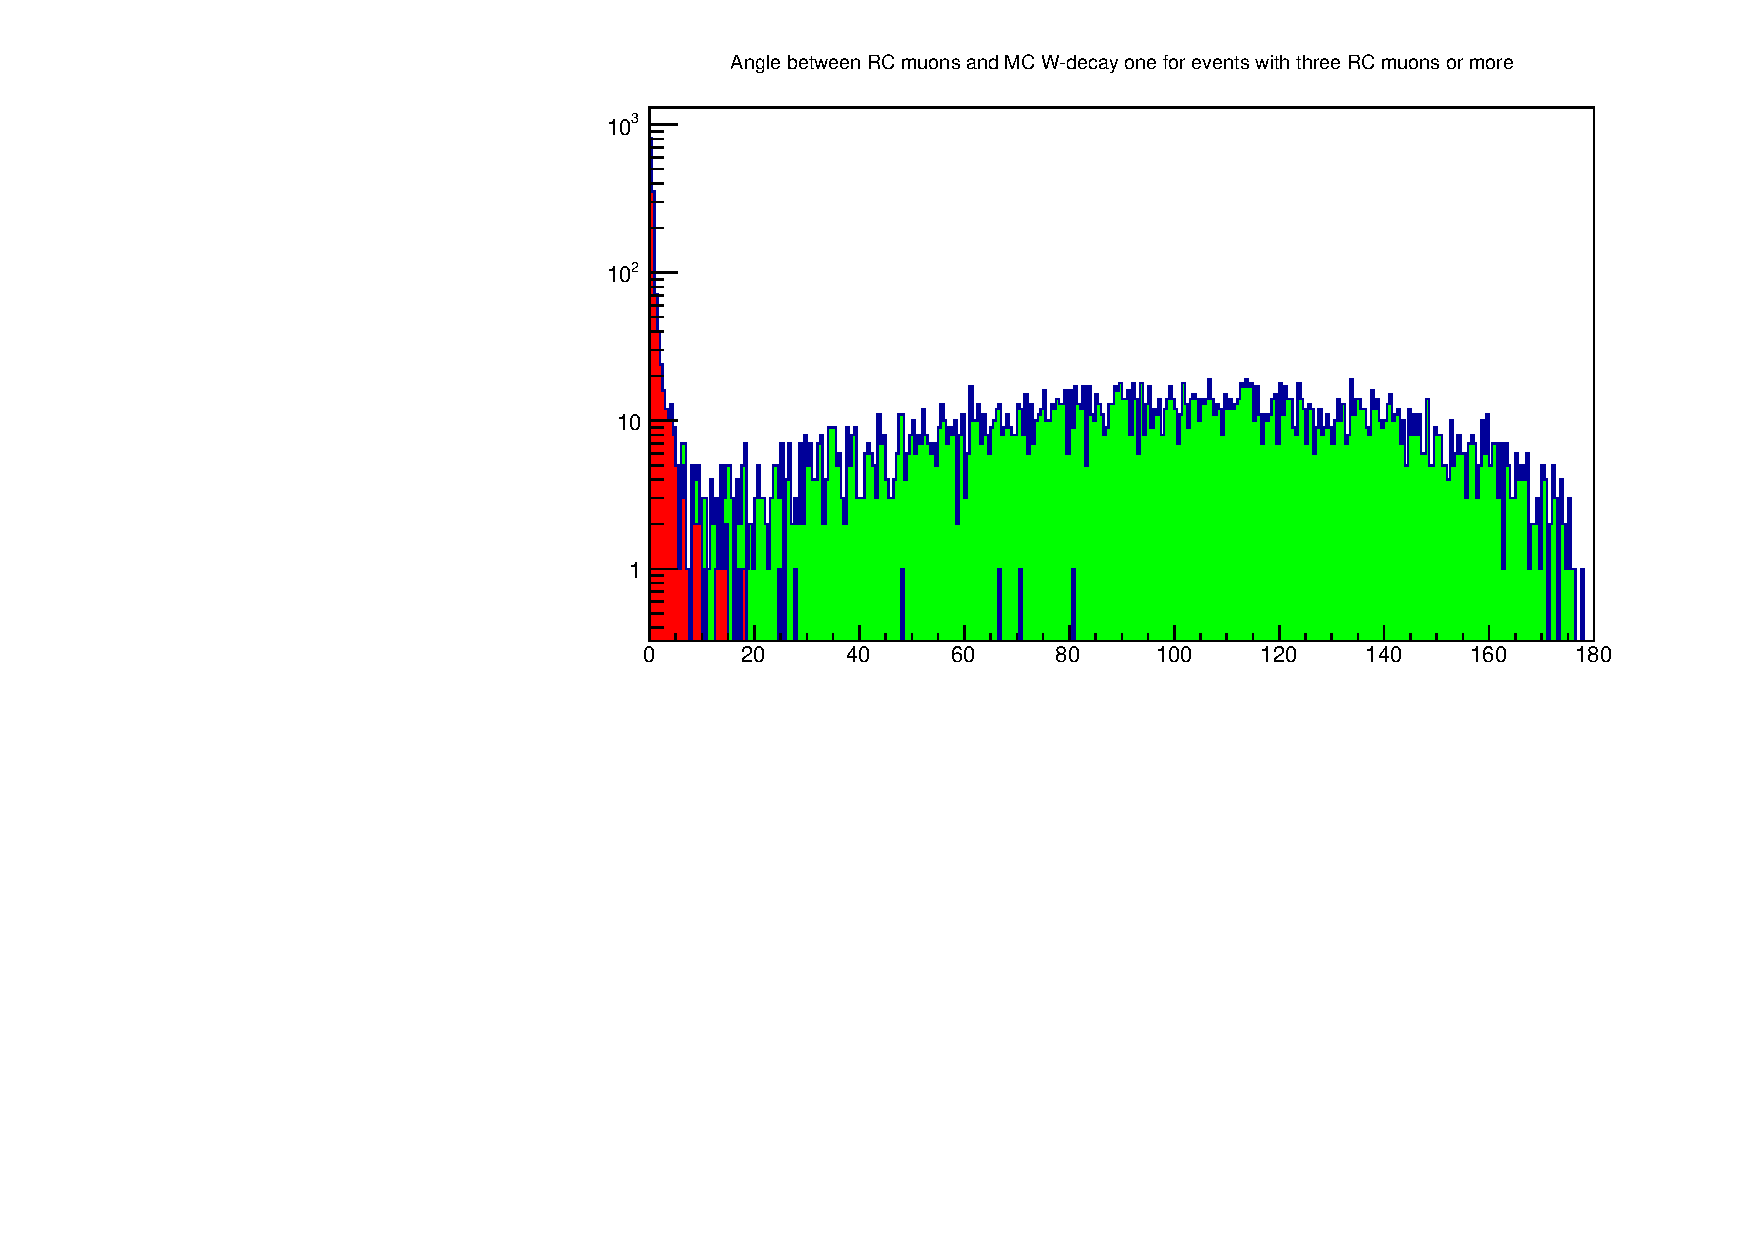
\includegraphics[scale=0.7]{04_muonsMatchAngleCutLog.pdf}
\caption{YLogscale is used for a better visualisation.}
\label{04_muonsMatchAngleCutLog}
\end{figure}

\begin{figure} [htp]
\centering
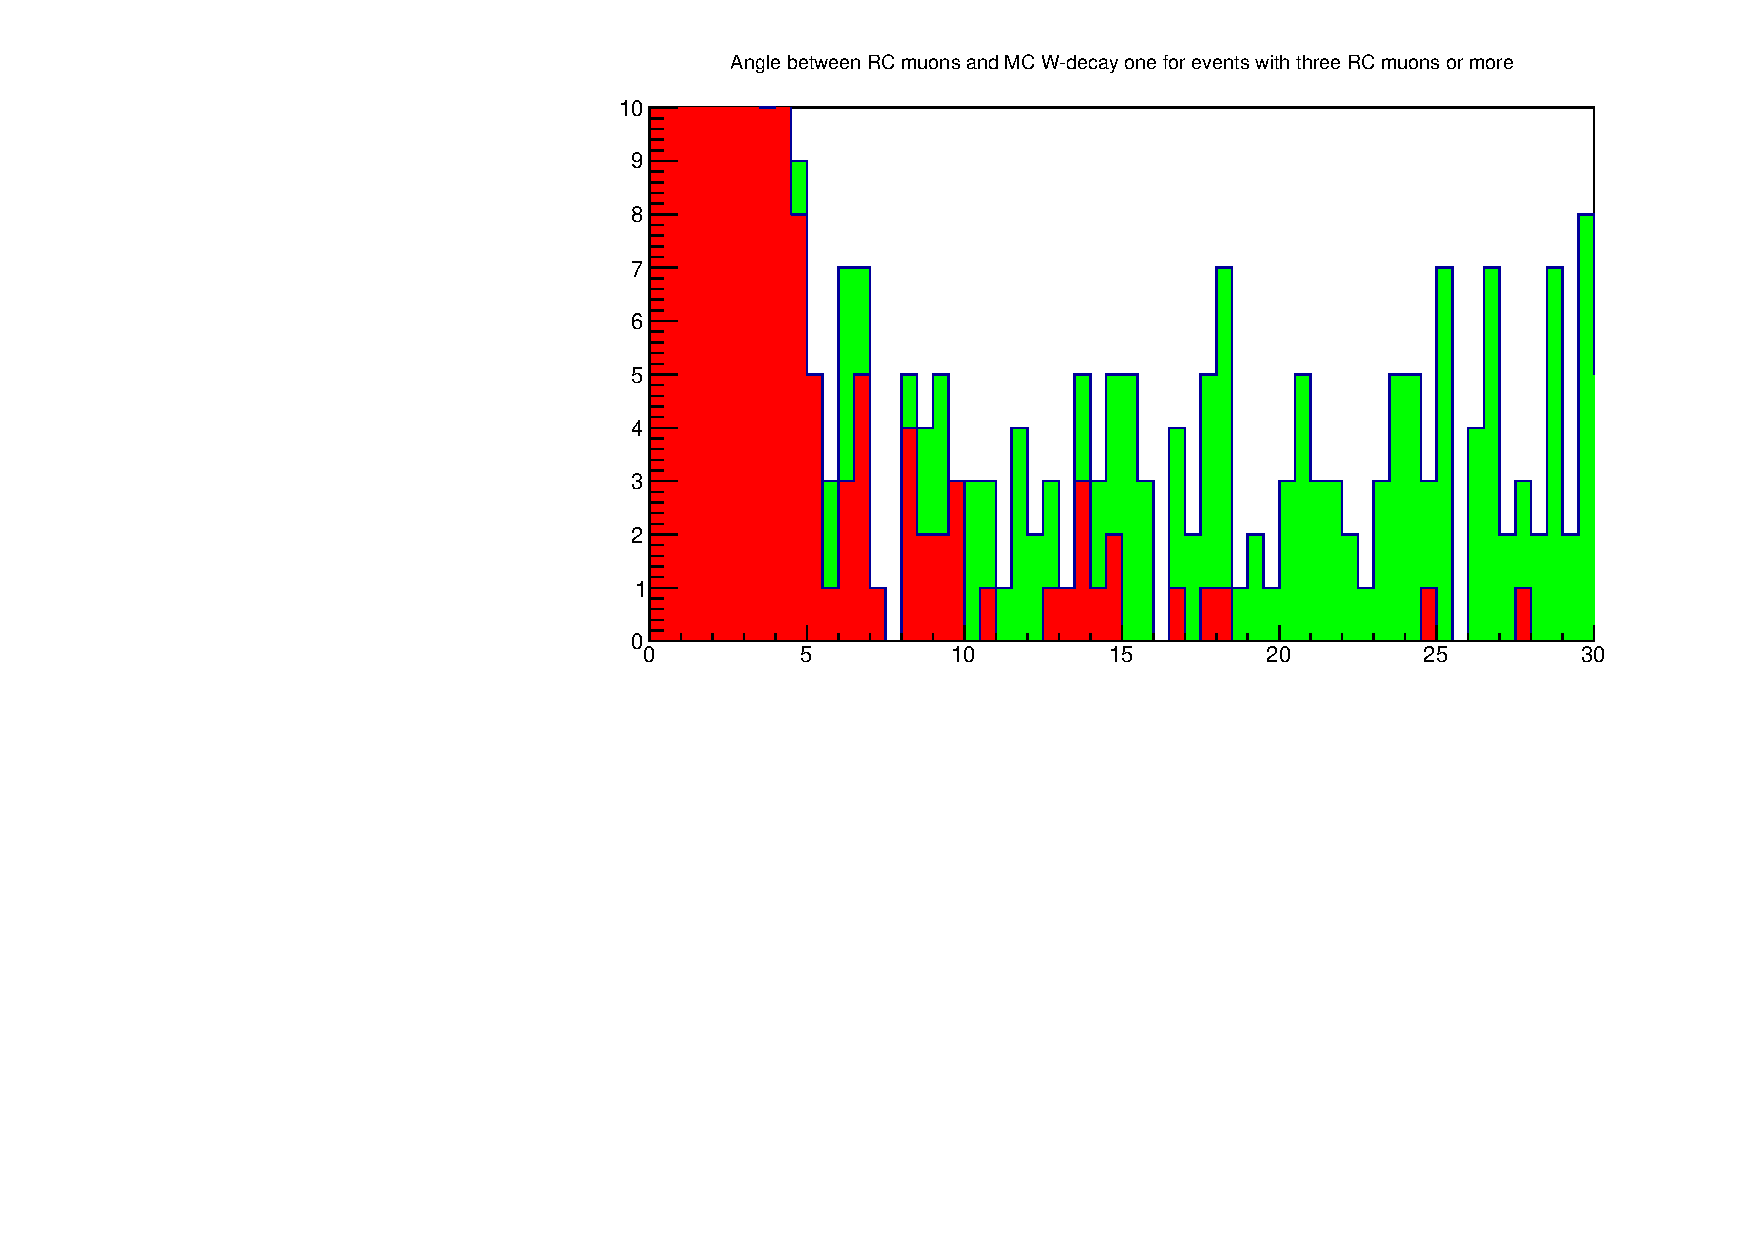
\includegraphics[scale=0.7]{04_muonsMatchAngleCut.pdf}
\caption{Zoom near the cut.}
\label{04_muonsMatchAngleCut}
\end{figure}

Looking at figure~\ref{04_muonsMatchAngleCut}, we decided to use $5.5^o$ as the maximum angle between two muons to say that they can match.

To sum up, we will say that a RC muon matches the W-MC muon if it is its closest RC muon and the angle between the two is smaller than $5.5^o$.

\subsection{14/08/15}

\textbf{Photons recovery}
We studied the phenomenon of photons emission by muons. This is nearly negligibile, but will increase its dimension in the electrons case, where it will be more difficult to study. We plotted the angular distribution of the photons with respect to the muons, separately for the muons that match the W-MC one and for the others. The results are plotted in figures~\ref{04_matchedMuonsPhotons}~and~\ref{04_notMatchedMuonsPhotons}.

\begin{figure} [htp]
\centering
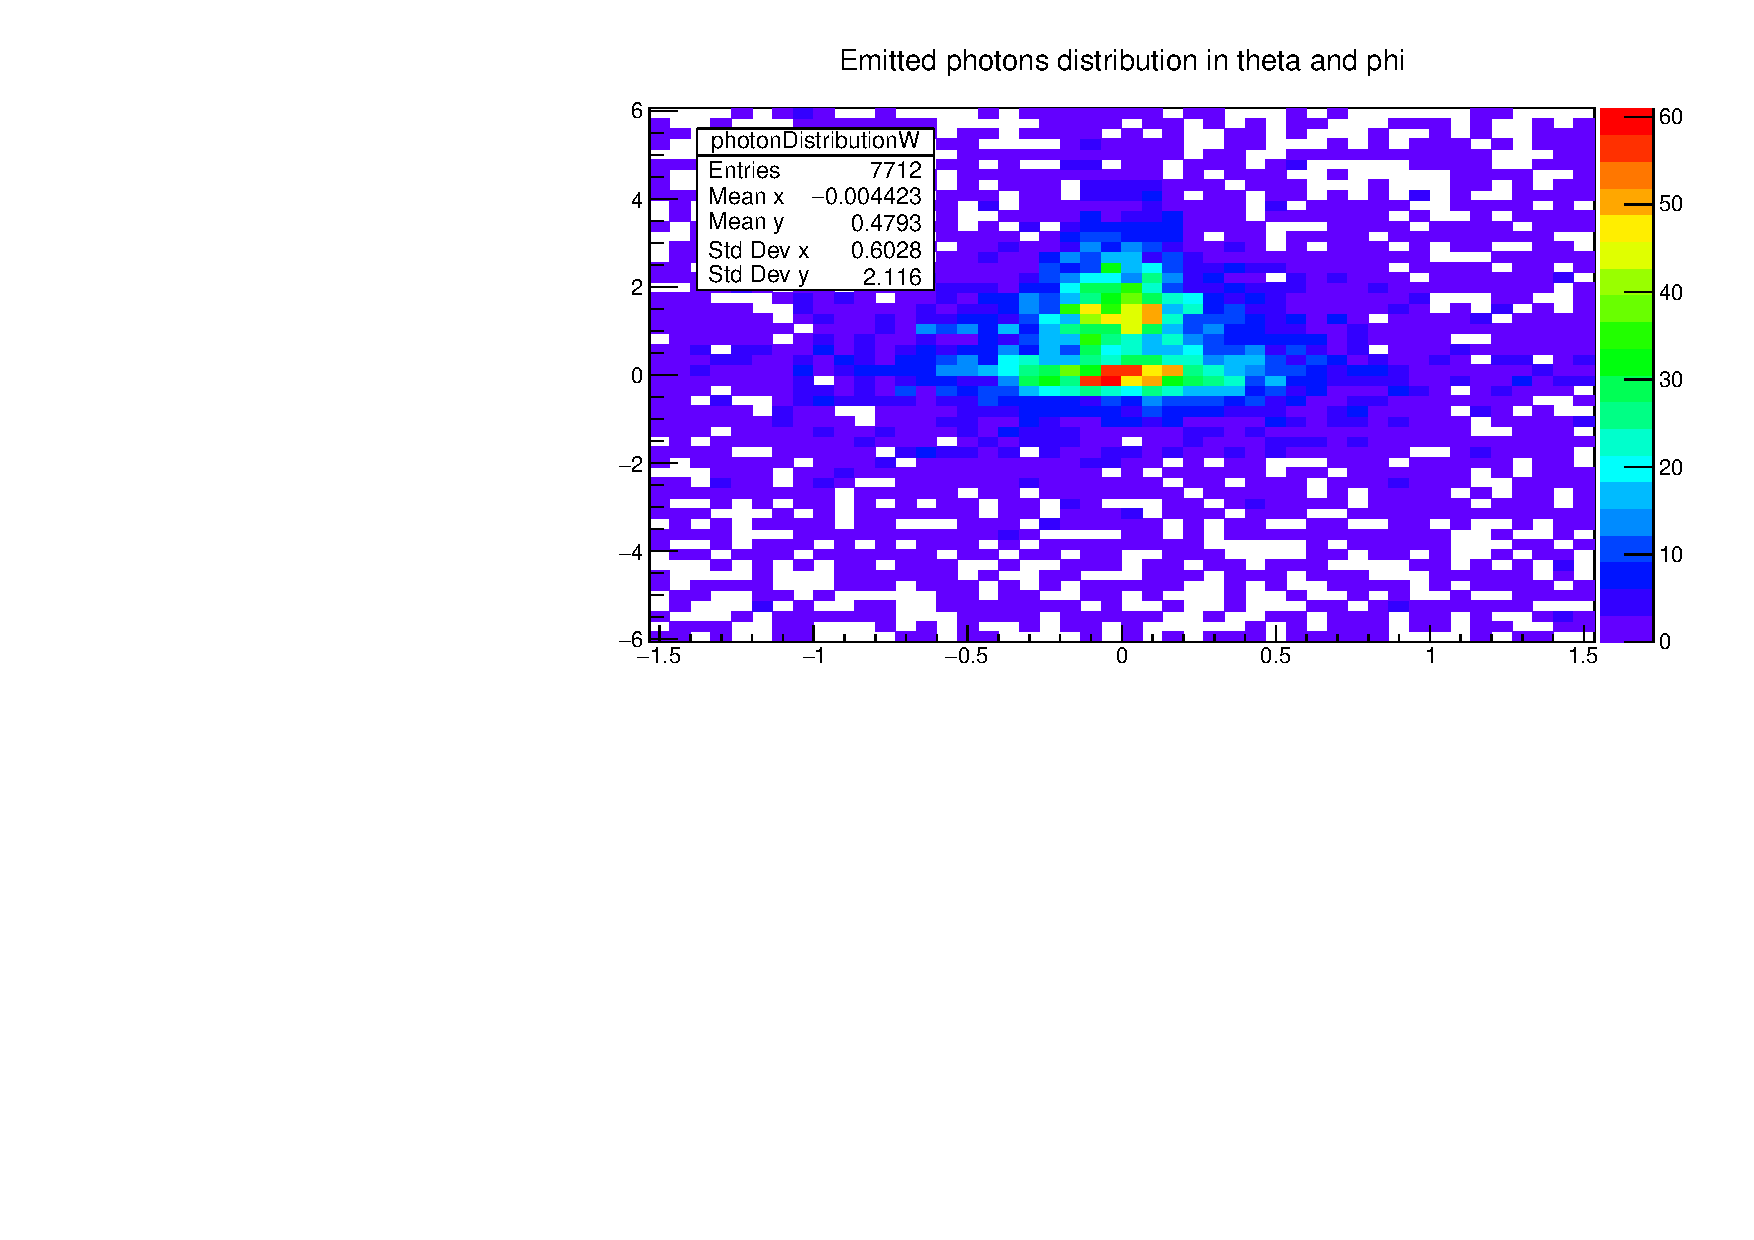
\includegraphics[scale=0.7]{04_matchedMuonsPhotons.pdf}
\caption{Angular distribution in $\theta$ and $\phi$ (degrees) of the photons with respect to the matched with W-MC muons.}
\label{04_matchedMuonsPhotons}
\end{figure}

\begin{figure} [htp]
\centering
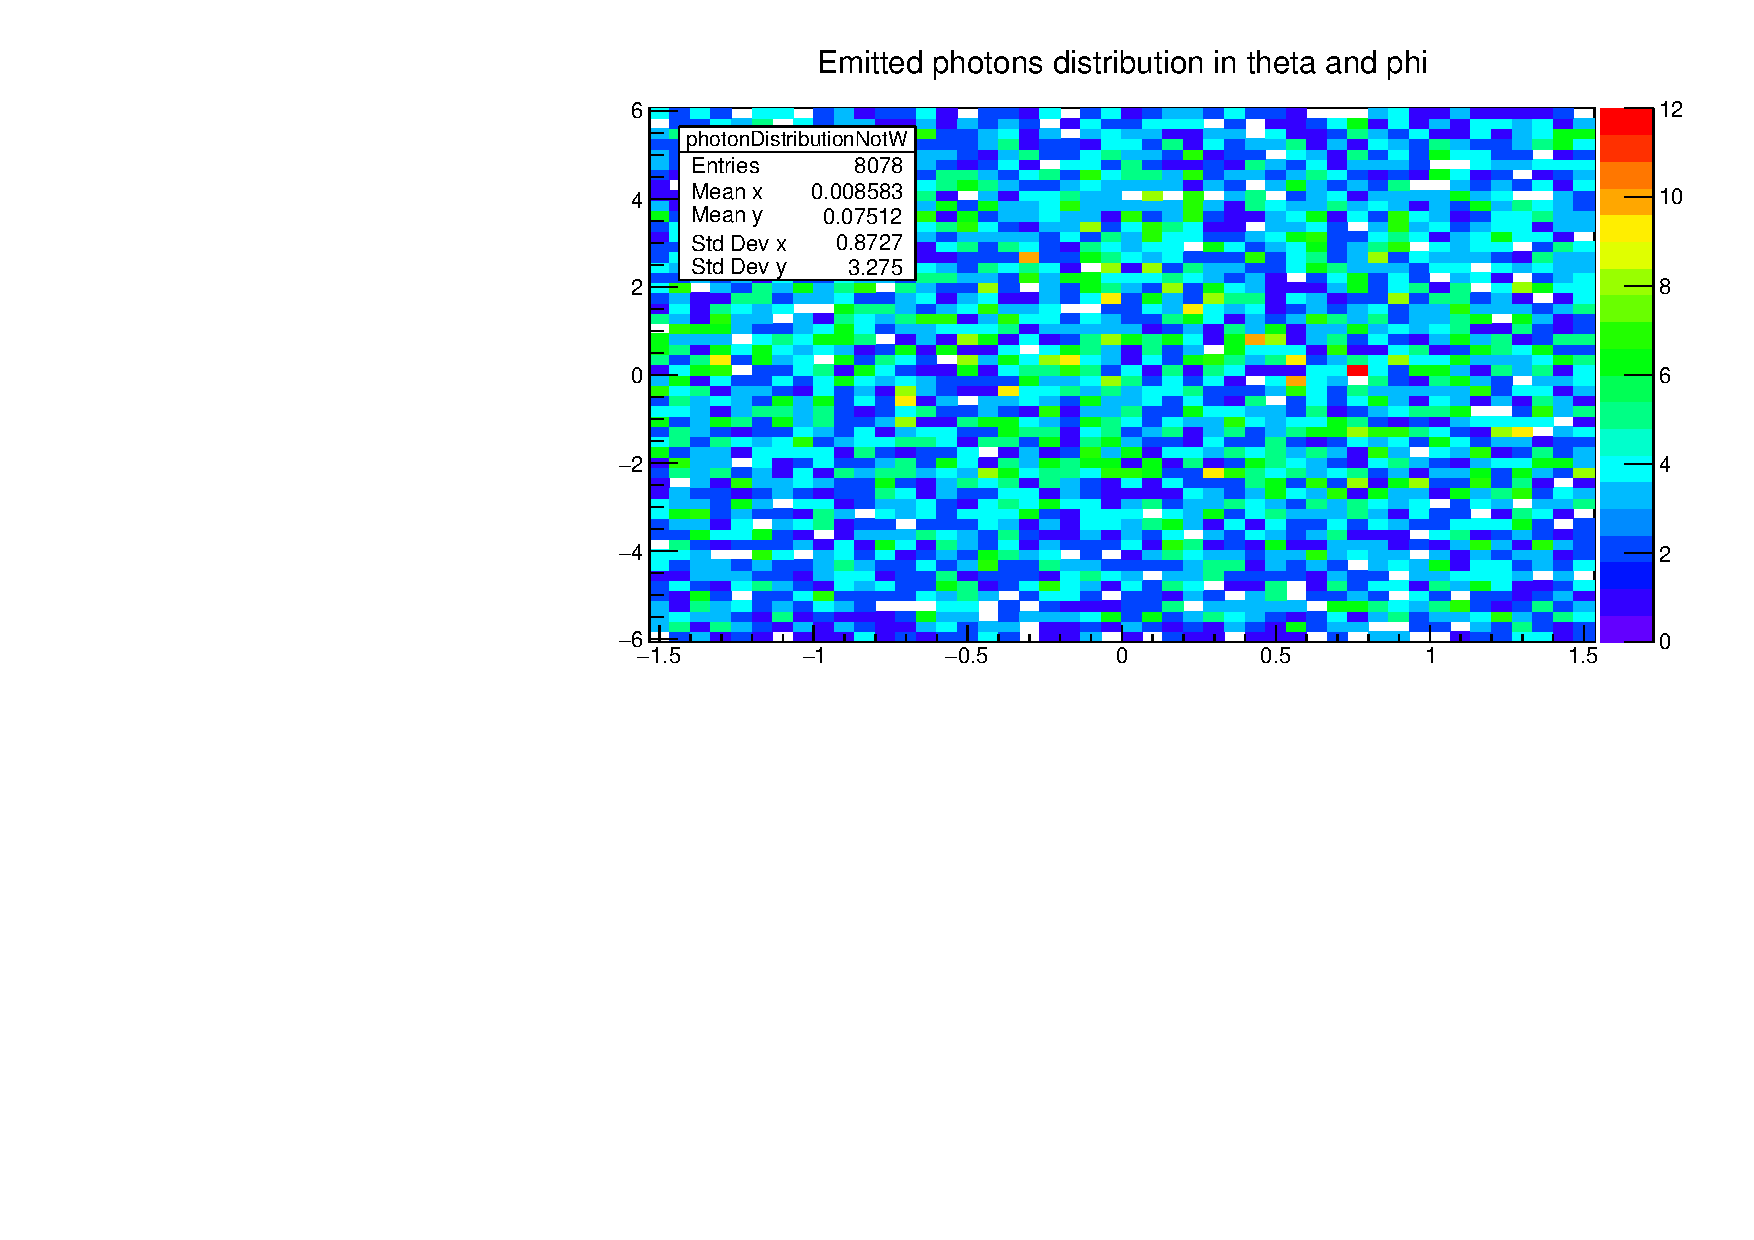
\includegraphics[scale=0.7]{04_notMatchedMuonsPhotons.pdf}
\caption{Angular distribution in $\theta$ and $\phi$ (degrees) of the photons with respect to the unmatched muons.}
\label{04_notMatchedMuonsPhotons}
\end{figure}

You can note the anisotropy of the distribution of the photons in $\phi$, due to the fact that the magnetic field present in the detection area makes the muons clockwise, so that they emit photons with $\phi > 0$. On the other hand, the muons that do not match the W-MC one are usually in a quark-jet, so that their photon distribution is nearly isotrope.
Our choice for the photons recovery, which is the first thing we make with our simulated data, is to sum to all the muons momenta the momenta of all the photons in the two rectangles $(\lvert\theta\rvert < 0.7, \lvert\phi\rvert < 0.8)$ and $(\lvert\theta\rvert < 0.35, -0.4<\phi < 3.5)$ around the muons.

The energy difference between RC and MC matched muons are plotted in figures~\ref{04_muonsBeforePhotonsRecovery}~and~\ref{04_muonsAfterPhotonsRecovery}, respectively before and after the photons recovery.

\begin{figure} [htp]
\centering
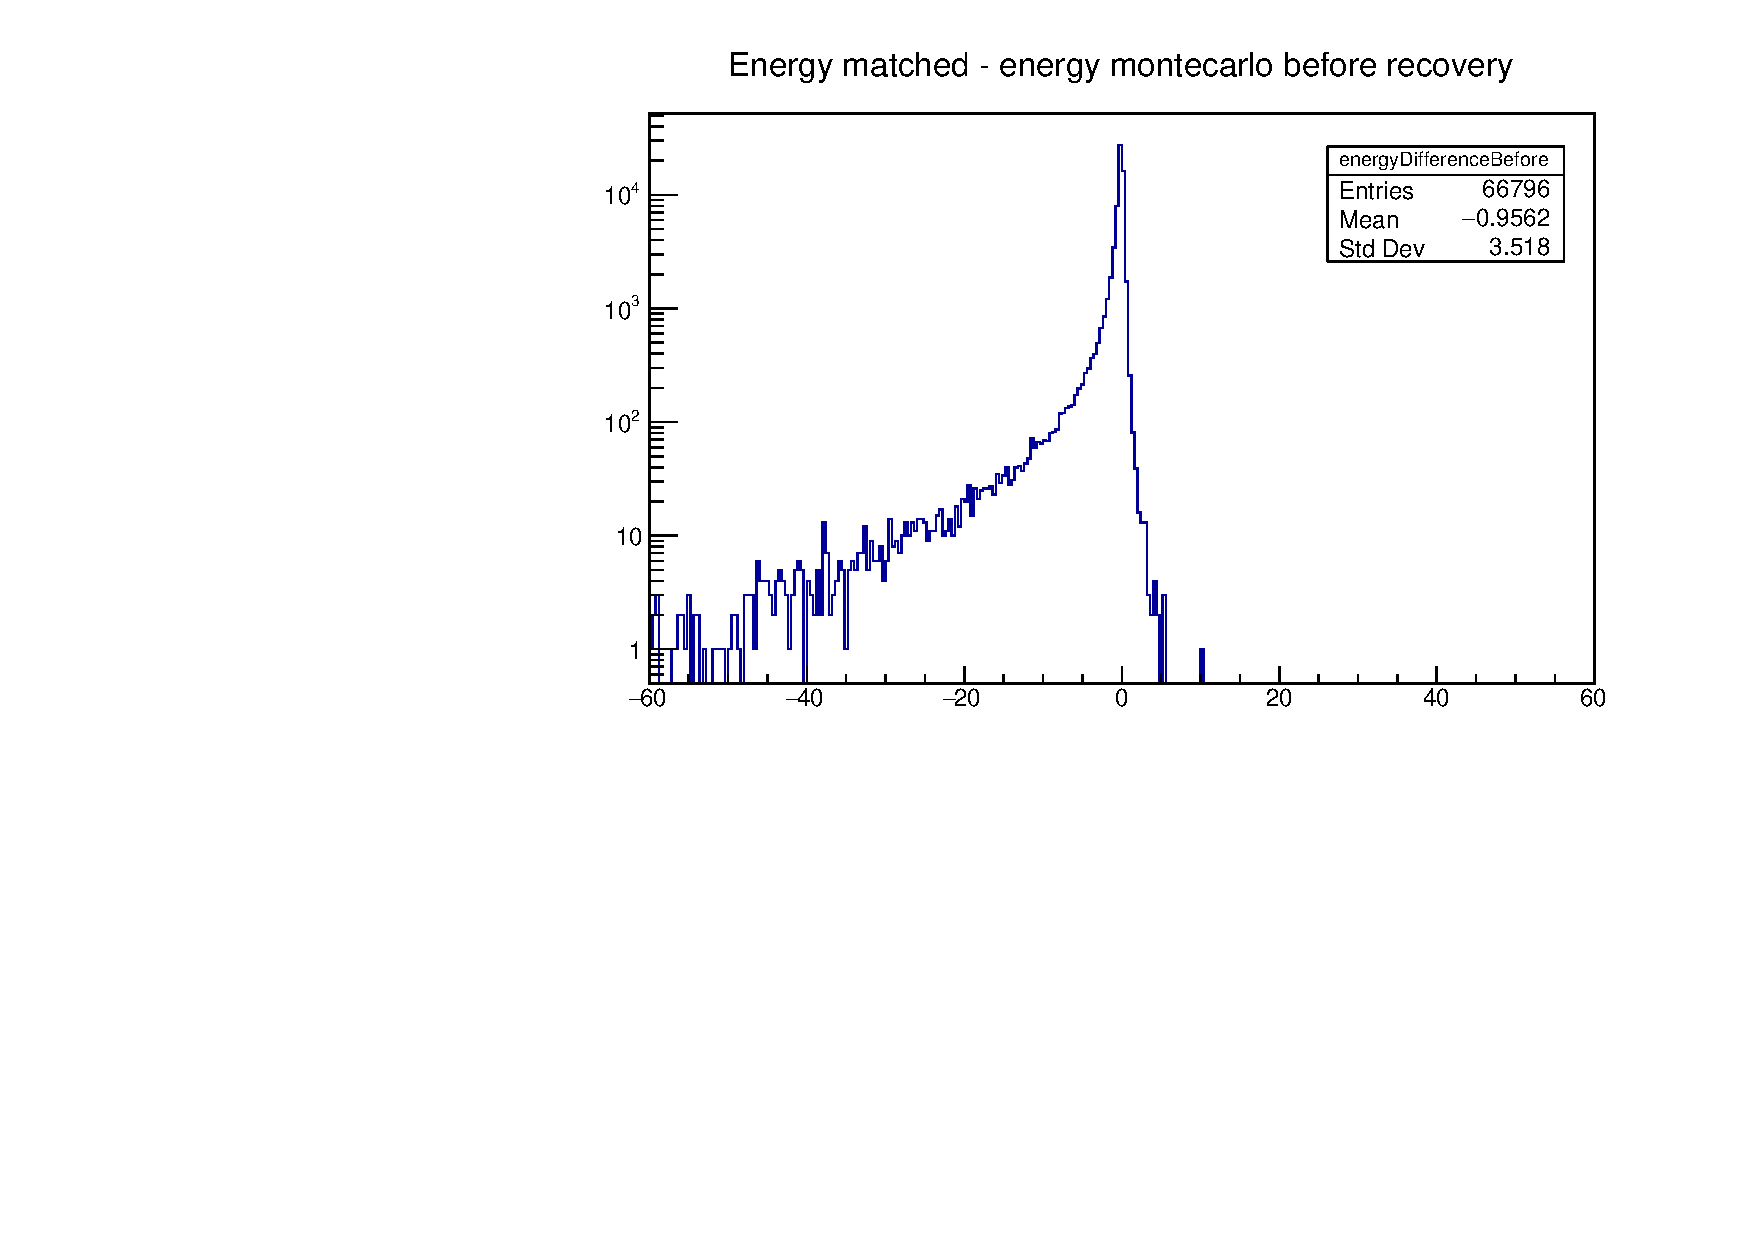
\includegraphics[scale=0.7]{04_muonsBeforePhotonsRecovery.pdf}
\caption{Energy differece between RC and MC matched muons before the photons recovery.}
\label{04_muonsBeforePhotonsRecovery}
\end{figure}

\begin{figure} [htp]
\centering
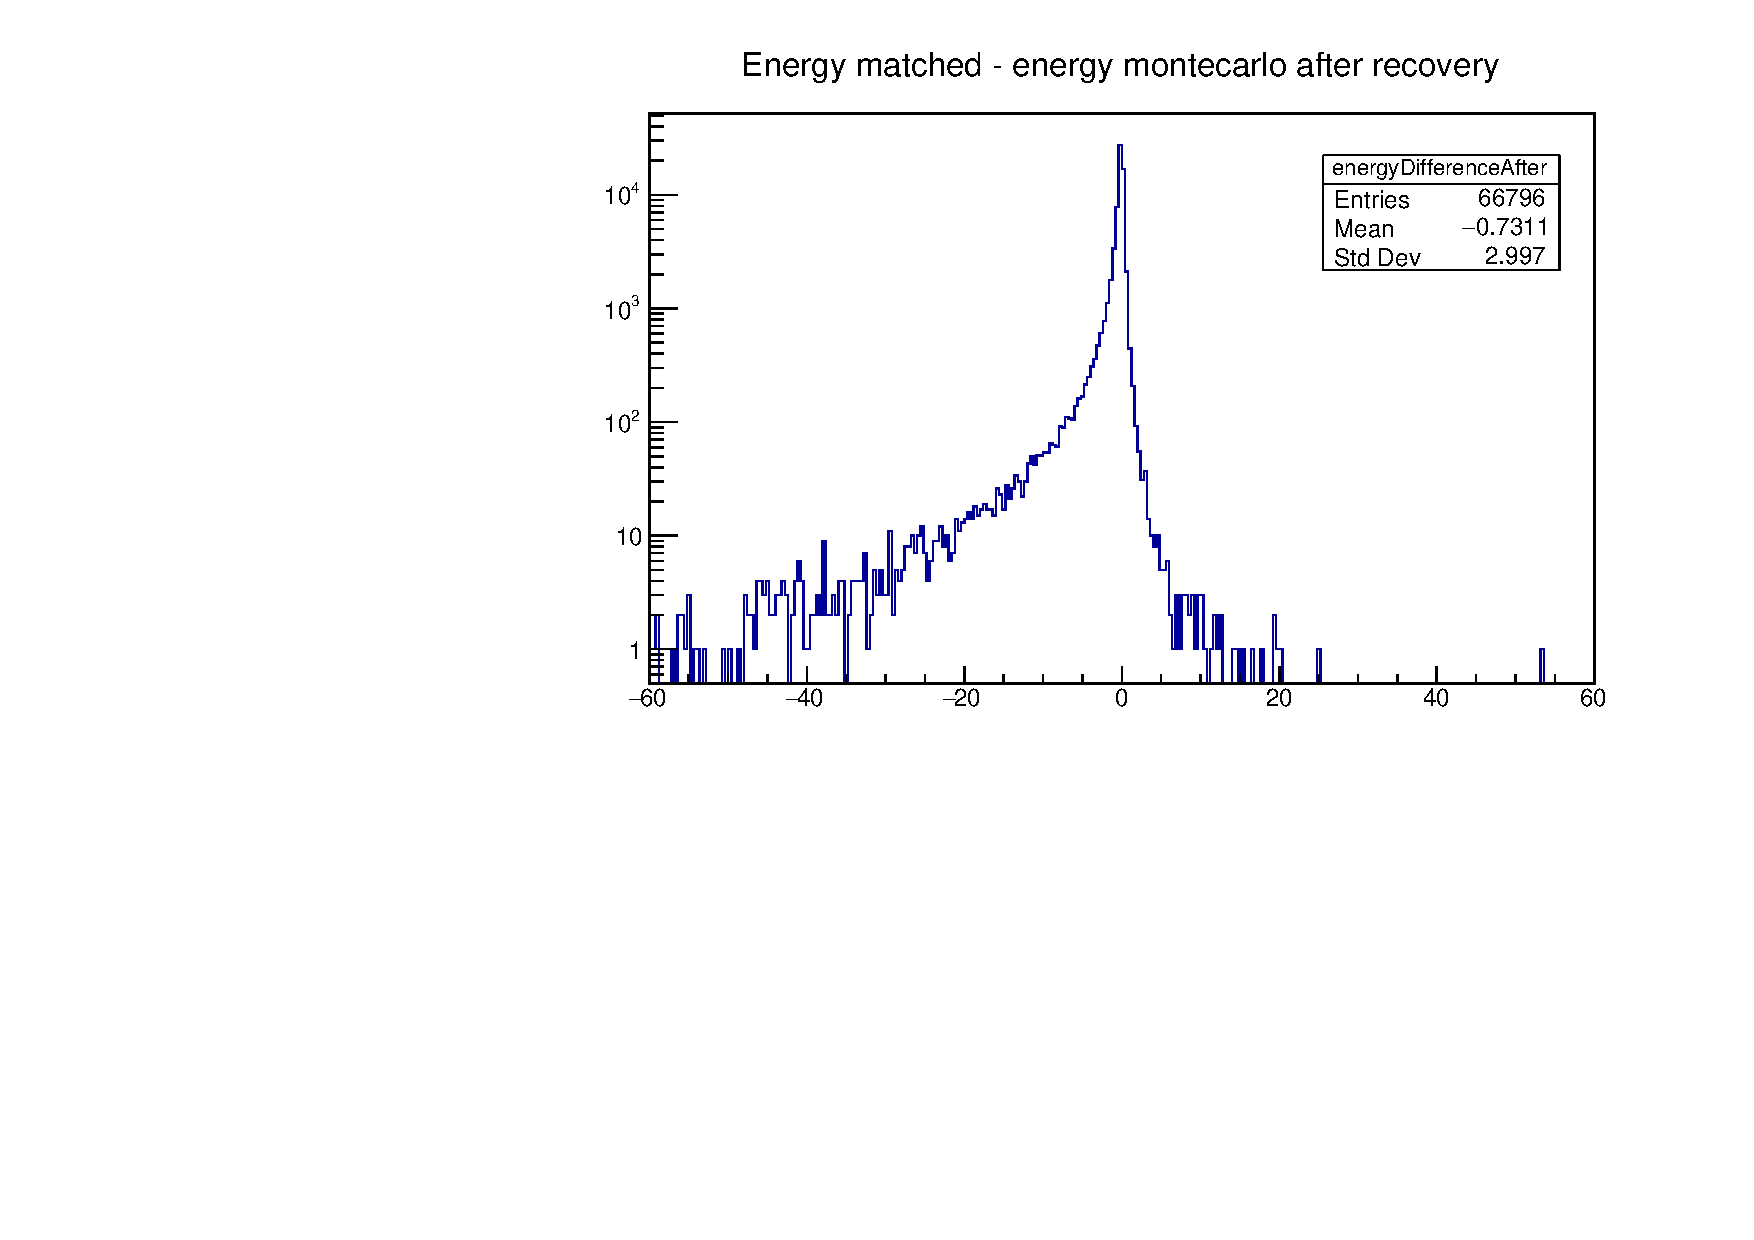
\includegraphics[scale=0.7]{04_muonsAfterPhotonsRecovery.pdf}
\caption{Energy differece between RC and MC matched muons after the photons recovery.}
\label{04_muonsAfterPhotonsRecovery}
\end{figure}

\textbf{Muon-jets exclusion}

We noticed that in the Tree producted by the Marlin program sometimes identifies muons as jets. In contrast, in our W-decay muon isolation algorithm we would like to consider as jets only those deriving from a quark. Therefore, we plotted the invariant mass of every muon with its closest jet, obtaining the results in figure~\ref{04_muonJetInvariantMass}. Looking at this histogram, we decided to exclude from our algorithms the jets which have an invariant mass (toghether with the muon in consideration) smaller than 11 GeV.

\begin{figure} [htp]
\centering
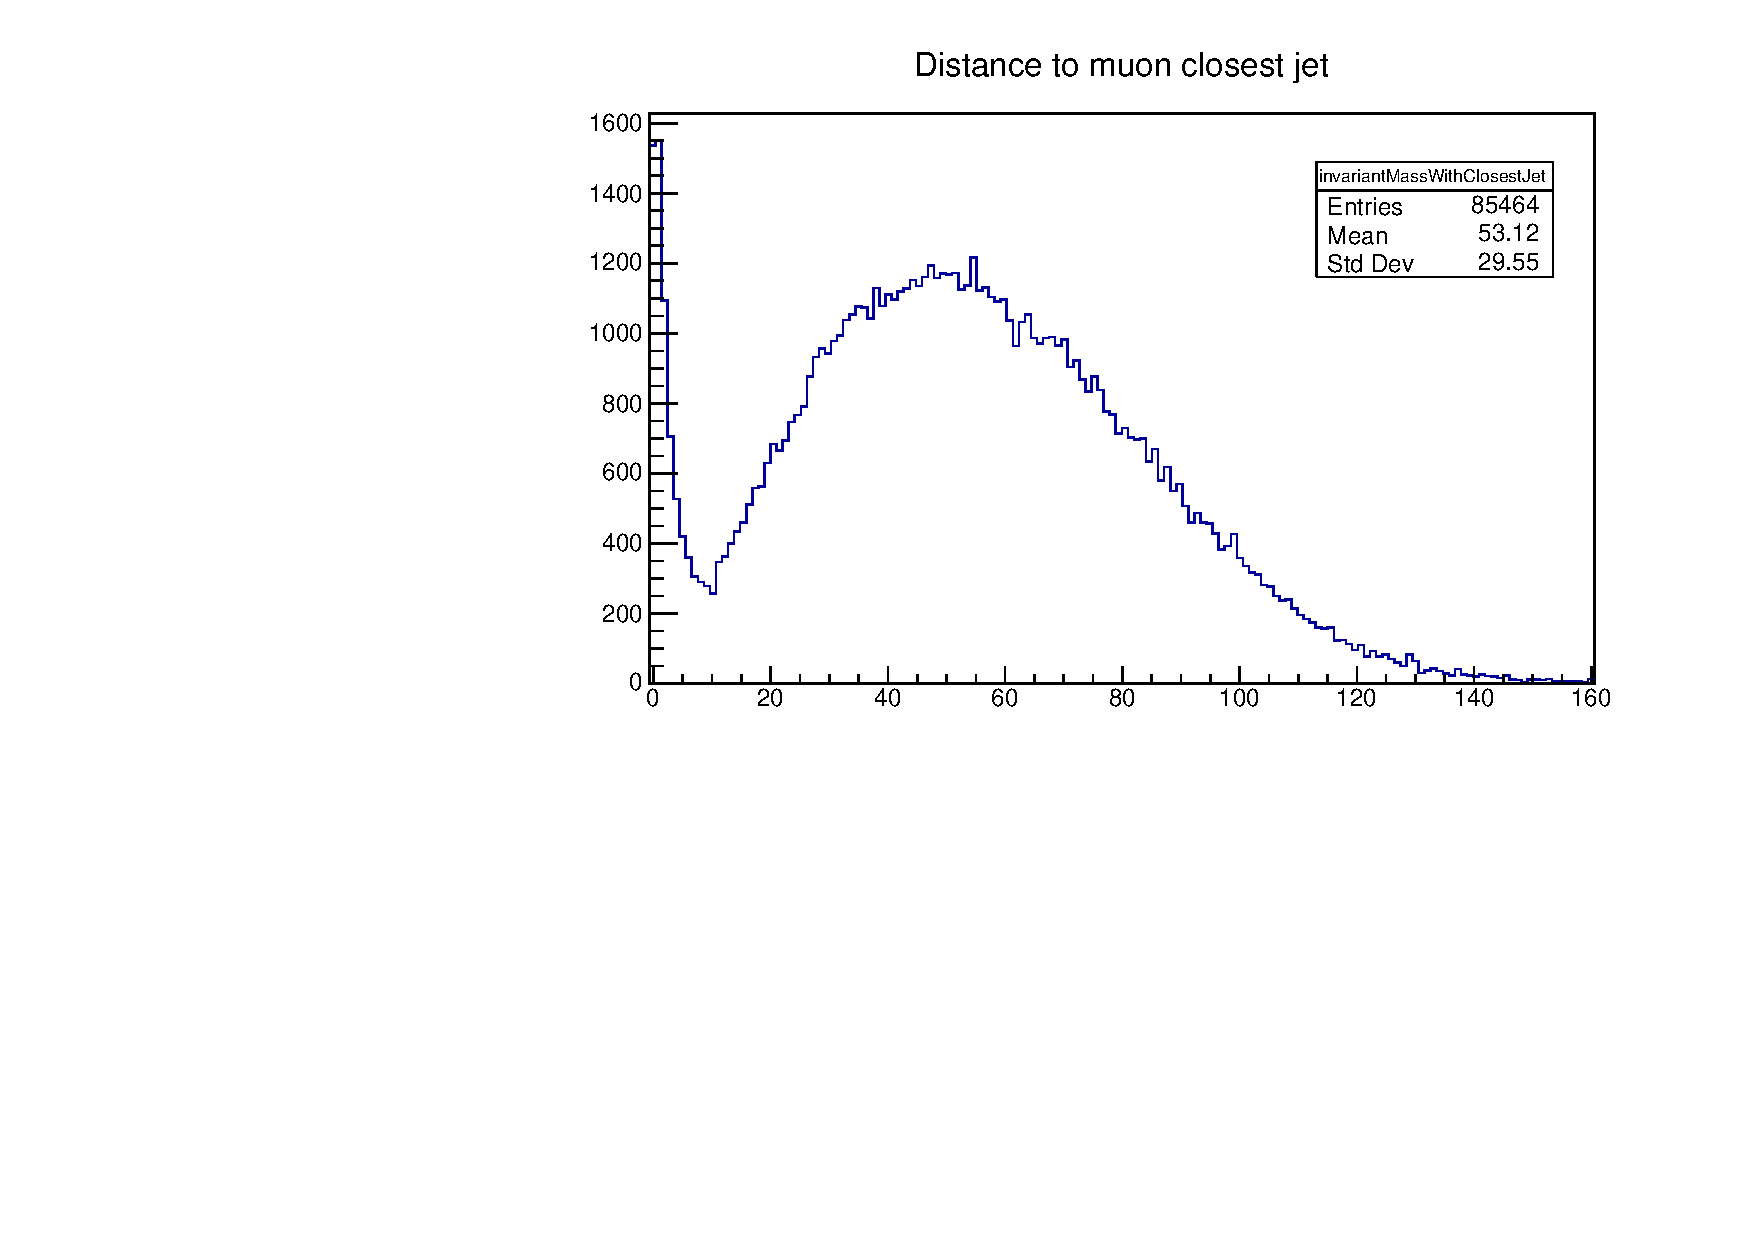
\includegraphics[scale=0.7]{04_muonJetInvariantMass.pdf}
\caption{Invariant mass of the muons with their closest jet (GeV).}
\label{04_muonJetInvariantMass}
\end{figure}
